\FloatBarrier
\section{Roadmap and conclusion}\label{sec:roadmap}

\subsection{Three generations}
\ac{1} is a first-generation part and its process and packaging choices are deliberately
conservative. The roadmap in Fig.~\ref{fig:roadmap} describes two follow-ons. \ac{2} moves to a
2 nm-class node, doubles the tile count to 128 and the L3 to 256 MB, and keeps the 65 W envelope;
the expected gain is 2.0$\times$ throughput at iso-power, mostly from density and from a wider
halo fabric. \ac{3} moves to an A14-class node with backside power and a 3D-stacked compute-on-SRAM
arrangement, targeting 240 TFLOPS at 70 W and a 512-member ensemble in one card.

The generational plan is not a clock-speed story. Each generation buys a larger ensemble, a larger
domain, or a longer forecast at the same energy; the frequency stays near 1.8--2.0 GHz because the
design is memory- and precision-bound rather than frequency-bound.

\begin{figure}[t]
\centering
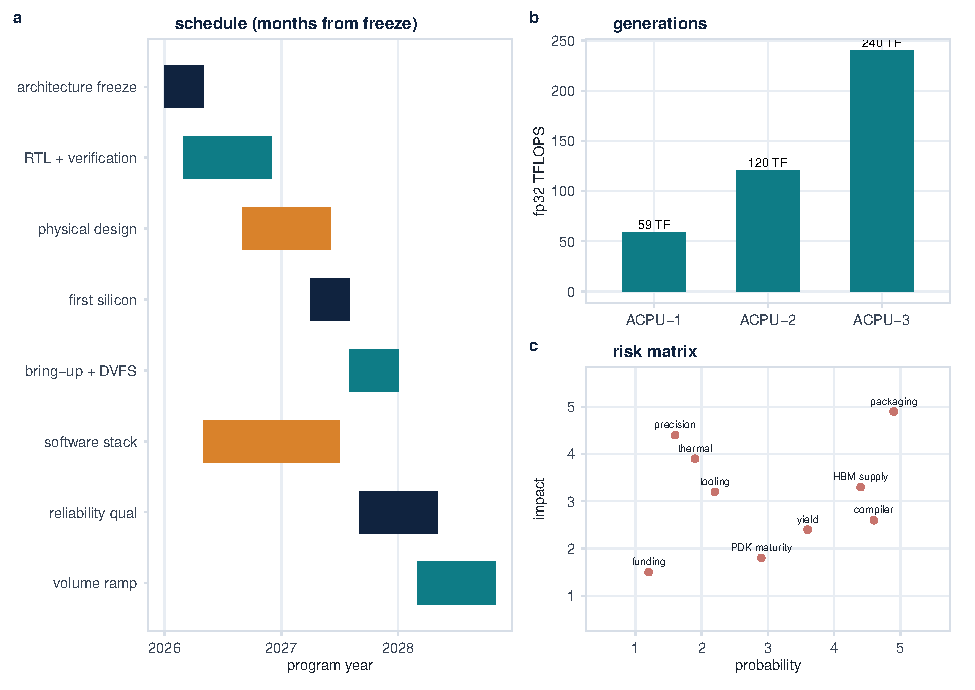
\includegraphics[width=\linewidth]{fig26_roadmap}
\caption{Roadmap. (a) 34-month programme from architecture freeze to volume ramp. (b) Three
generations. (c) Risk matrix; packaging, thermal and precision validation are the high-impact
items.}
\label{fig:roadmap}
\end{figure}

\subsection{Programme risks}
The risk matrix in Fig.~\ref{fig:roadmap}(c) ranks packaging and thermal as the highest-impact
items. Hybrid bonding of two 64 MB dies onto a 287.6 mm$^2$ compute die is the least mature step in
the flow; the fallback is a single 96 MB L3 die on the interposer, which costs 20\% of the L3
bandwidth and postpones the second-generation stack. HBM supply is a commercial risk rather than a
technical one. Precision validation on a full model is the highest technical risk with the lowest
mitigation cost: it is a software experiment that can run before tape-out.

\subsection{Conclusion}
This report specified a processor for atmospheric chaotic computation and evaluated it against the
machine that the field currently uses. The design is organised around three observations:
ensembles are the natural parallel dimension, stencils are memory problems, and forecast error is
chaotic rather than arithmetic. The resulting chip is small, air-cooled and cheap; it sustains
41.9 TFLOPS at 57 W, runs a 64-member 24-hour forecast in two minutes, and is projected to use
\ACRatioDay$\times$ less energy per forecast-and-analysis day than an H100 at comparable
wall-clock.

The number that matters is not the ratio itself. It is that the ratio survives the sensitivity
analysis, survives the idealised-GPU bound, and decomposes into mechanisms that can be measured on
real silicon. A 3.9$\times$ advantage at 100\% GPU utilisation is still a reason to build the
machine; a 9.3$\times$ advantage at realistic utilisation is a reason to build it now.

The next step is not another simulation. It is a two-week experiment on an H100 that runs the ten
kernels of Table~\ref{tab:kernels} at state-of-the-art efficiency and measures joules per
delivered forecast. That measurement would either validate the thesis or kill it, and either
outcome is worth more than a third decimal place in a projection.
